%%%%%%%%%%%%%%%%%%%%%%%%%%%%%%%%%%%%%%%%%%%%%%%%
% Template TCMN data sheet version 3
% 
% Alberto Sanchez asanchezrodelgo@ifc.org Dec 2015
%%%%%%%%%%%%%%%%%%%%%%%%%%%%%%%%%%%%%%%%%%%%%%%%
\documentclass{article}\usepackage[]{graphicx}\usepackage[]{color}
%% maxwidth is the original width if it is less than linewidth
%% otherwise use linewidth (to make sure the graphics do not exceed the margin)
\makeatletter
\def\maxwidth{ %
  \ifdim\Gin@nat@width>\linewidth
    \linewidth
  \else
    \Gin@nat@width
  \fi
}
\makeatother

\definecolor{fgcolor}{rgb}{0.345, 0.345, 0.345}
\newcommand{\hlnum}[1]{\textcolor[rgb]{0.686,0.059,0.569}{#1}}%
\newcommand{\hlstr}[1]{\textcolor[rgb]{0.192,0.494,0.8}{#1}}%
\newcommand{\hlcom}[1]{\textcolor[rgb]{0.678,0.584,0.686}{\textit{#1}}}%
\newcommand{\hlopt}[1]{\textcolor[rgb]{0,0,0}{#1}}%
\newcommand{\hlstd}[1]{\textcolor[rgb]{0.345,0.345,0.345}{#1}}%
\newcommand{\hlkwa}[1]{\textcolor[rgb]{0.161,0.373,0.58}{\textbf{#1}}}%
\newcommand{\hlkwb}[1]{\textcolor[rgb]{0.69,0.353,0.396}{#1}}%
\newcommand{\hlkwc}[1]{\textcolor[rgb]{0.333,0.667,0.333}{#1}}%
\newcommand{\hlkwd}[1]{\textcolor[rgb]{0.737,0.353,0.396}{\textbf{#1}}}%

\usepackage{framed}
\makeatletter
\newenvironment{kframe}{%
 \def\at@end@of@kframe{}%
 \ifinner\ifhmode%
  \def\at@end@of@kframe{\end{minipage}}%
  \begin{minipage}{\columnwidth}%
 \fi\fi%
 \def\FrameCommand##1{\hskip\@totalleftmargin \hskip-\fboxsep
 \colorbox{shadecolor}{##1}\hskip-\fboxsep
     % There is no \\@totalrightmargin, so:
     \hskip-\linewidth \hskip-\@totalleftmargin \hskip\columnwidth}%
 \MakeFramed {\advance\hsize-\width
   \@totalleftmargin\z@ \linewidth\hsize
   \@setminipage}}%
 {\par\unskip\endMakeFramed%
 \at@end@of@kframe}
\makeatother

\definecolor{shadecolor}{rgb}{.97, .97, .97}
\definecolor{messagecolor}{rgb}{0, 0, 0}
\definecolor{warningcolor}{rgb}{1, 0, 1}
\definecolor{errorcolor}{rgb}{1, 0, 0}
\newenvironment{knitrout}{}{} % an empty environment to be redefined in TeX

\usepackage{alltt}
%%%%%%%%%%%%%% package declaration %%%%%%%%%%%%%%%%%%%%%
\usepackage[top=0.3in, bottom=0.1in, left=0.5in, right=0.6in]{geometry}
\usepackage{graphicx} % to load images
\usepackage[export]{adjustbox} % add alignment to includegraphics
\usepackage[font=small]{caption}
\usepackage{xcolor} % color text
\usepackage{tabularx} % to adjust table width, etc. 
\usepackage{titlesec} % format titles and headers
\usepackage{sectsty} % format sections & subsections
\usepackage{booktabs} % For \toprule, \midrule and \bottomrule
\usepackage[colorlinks = true,
            linkcolor = blue,
            urlcolor  = blue,
            citecolor = blue,
            anchorcolor = blue]{hyperref} % to include hyperlinks in the doc
\sectionfont{\fontsize{16}{15}\selectfont\raggedright} % formats title newsletter (section) 
\subsectionfont{\fontsize{14}{12}\selectfont\raggedright} % formats title newsletter (section)
%%%%%%%%%%%%%%%%%%%%%%%%%%%%%%%%%%%%%%%%%%%%%%%%%%%%%%%%%%%%%%%%%%%%%%%%%%%%%%%%%%%
%
%%%%%%%%%%%%%%%%%%%%%%%%%%%%%%%%%%%%% BEGIN DOCUMENT %%%%%%%%%%%%%%%%%%%%%%%%%%%%%%
\IfFileExists{upquote.sty}{\usepackage{upquote}}{}
\begin{document}

%

%%%%%%%%%%%%%%%% PAGE 1 %%%%%%%%%%%%%%%%%%%
%World Bank logo and TCMN branding
\begin{figure}
  \vspace{-3ex} % move up this figure
  \hspace{-7ex} % move left this figure
  \includegraphics[width=5cm]{/Users/asanchez3/shinyTCMN/www/wb_logo_background.png}
\end{figure}
\begin{figure}
  \begin{minipage}[t]{0.99\textwidth} % top section
      \vspace{-30ex}
      \hspace{-2ex}
      \raggedright{\includegraphics[width=5.5cm,right]{/Users/asanchez3/shinyTCMN/www/TC_snapshots_data.png}}
  %  {\color{white!70!black}\noindent\makebox[\linewidth]{\rule{20cm}{0.3pt}}} % horiz line
  \end{minipage}
\end{figure}
%
%%%% Macro Indicators
\begin{minipage}[t]{0.99\textwidth} % top section
  \vspace{-1.5cm}
  \begin{minipage}[c]{0.36\textwidth} 
    \begin{minipage}[c]{0.28\textwidth} % flag
      \includegraphics[width=1.2cm,height=1.2cm]{/Users/asanchez3/shinyTCMN/www/TJ.png}
    \end{minipage}
    \begin{minipage}[c]{0.70\textwidth} % Country name
      \section*{\color{blue!40!black}Tajikistan}
    \end{minipage}
  \end{minipage}
  \begin{minipage}[c]{0.63\textwidth} % key macro table 
    % Table 1
    \centering
    \resizebox{\textwidth}{!}{
% latex table generated in R 3.2.2 by xtable 1.7-4 package
% Wed May 25 16:26:55 2016
{\LARGE
\begin{tabular}{>{\centering}p{1.5in}>{\centering}p{1.5in}>{\centering}p{1.5in}>{\centering}p{1.5in}>{\centering}p{1.5in}>{\centering}p{1.5in}>{\centering}p{1.5in}l}
  GDP (US\$ billions) (2017) & Population (millions) (2017) & Land area (sq. km) (2015) & Income per capita (current US\$) (2017) & Poverty rate (2009) \large{[1]} & Unemployment rate (2016) & Ease of Doing Business Rank (2016) &  \\ 
        9.7 &       8.9 & 139,960.0 &   1,096.1 &       4.7 &        NA &     132.0 &  \\ 
  \end{tabular}
}

    }
  \end{minipage}  
\end{minipage} % end top section

\begin{minipage}[b]{0.99\textwidth} % macro indicators main table
  \begin{minipage}[t]{0.99\textwidth}

    \begin{minipage}[c]{0.875\textwidth}
      \begin{flushleft}  
      {\color{white!30!blue} \textbf{\small Macro Indicators}}
      \end{flushleft} 
      \vspace*{-0.4cm}
      % Table 2
      \centering
      \resizebox{\textwidth}{!}{
% latex table generated in R 3.2.2 by xtable 1.7-4 package
% Wed May 25 16:26:55 2016
{\Large
\begin{tabular}{>{\raggedright}p{6in}r>{\raggedleft}p{0.8in}>{\raggedleft}p{0.8in}>{\raggedleft}p{0.8in}>{\raggedleft}p{0.8in}>{\raggedleft}p{0.8in}l}
  & Avg 2003-2012 & 2013 & 2014 & 2015 & 2016 & 2017 &  \\ 
  \hline
GDP growth (annual \%) &   8.08 &   7.40 &   6.70 &   4.20 &   4.80 &   5.55 &  \\ 
  Current account balance &  -3.30 &  -2.81 &  -7.93 &  -6.30 &  -5.96 &  -5.89 &  \\ 
  Fiscal balance (\% of GDP) &  -2.87 &  -1.01 &  -0.48 &  -1.36 &  -1.91 &  -1.85 &  \\ 
  Remittances, received (\% of GDP) \large{[1]} &  34.28 &  49.59 &  43.01 & --- & --- & --- &  \\ 
  General government gross debt \large{[3]} &  43.72 &  29.18 &  28.34 &  35.91 &  50.27 & --- &  \\ 
  Real Effective Exchange Rate (2010=100) &  85.61 & 148.13 & 164.98 & 160.79 & 157.94 & 158.09 &  \\ 
  Consumer Price Index, annual percent change &  12.85 &   5.03 &   6.18 &   8.50 &   7.50 &   7.00 &  \\ 
  \end{tabular}
}

      }
    \end{minipage}
    \begin{minipage}[c]{0.11\textwidth}
      \vspace*{+0.8cm}


{\centering 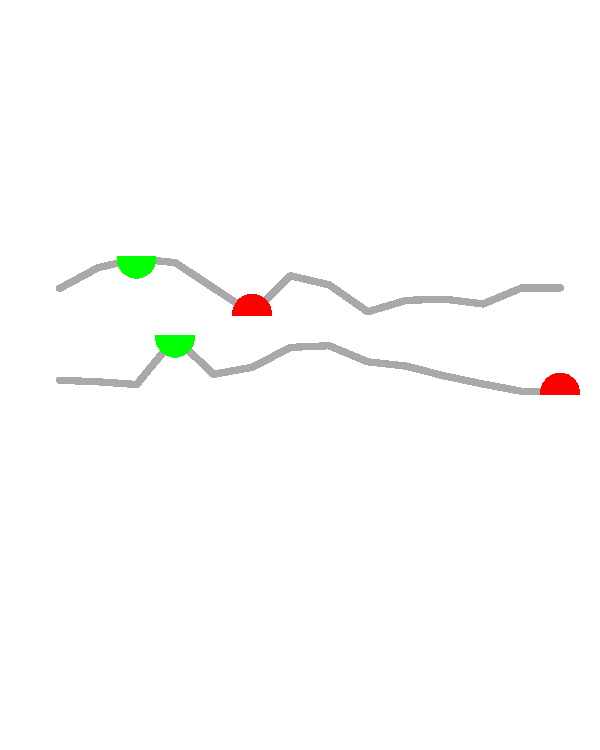
\includegraphics[width=\maxwidth]{figure/createSparklines_macro-1} 

}



      \vspace*{-0.5cm}
    \end{minipage}
    
    %\vspace*{-0.4cm}
    \begin{minipage}[c]{0.875\textwidth}
      \begin{flushleft}  
      {\color{white!30!blue} \textbf{\small Investment indicators}}
      \end{flushleft} 
      \vspace*{-0.4cm}
      % Table 2
      \centering
      \resizebox{\textwidth}{!}{
% latex table generated in R 3.2.2 by xtable 1.7-4 package
% Wed May 25 16:26:55 2016
{\Large
\begin{tabular}{>{\raggedright}p{6in}r>{\raggedleft}p{0.8in}>{\raggedleft}p{0.8in}>{\raggedleft}p{0.8in}>{\raggedleft}p{0.8in}>{\raggedleft}p{0.8in}l}
  & Avg 2003-2012 & 2013 & 2014 & 2015 & 2016 & 2017 &  \\ 
  \hline
Gross domestic investment (\% GDP) &  6.3 &  5.8 &  5.7 &  5.9 &  6.3 &  6.4 &  \\ 
  Gross domestic investment, of w: Private investment (\% GDP) \large{[1]} & 17.7 & 19.1 & --- & --- & --- & --- &  \\ 
  Inward FDI (\% of GDP) \large{[2]} &  4.9 &  1.2 &  2.8 & --- & --- & --- &  \\ 
  Inward FDI, \% of private investment \large{[2]} & 33.4 &  6.7 &   NA & --- & --- & --- &  \\ 
  \end{tabular}
}

      }
    \end{minipage}
    \begin{minipage}[c]{0.11\textwidth}
      \vspace*{+0.8cm}


{\centering 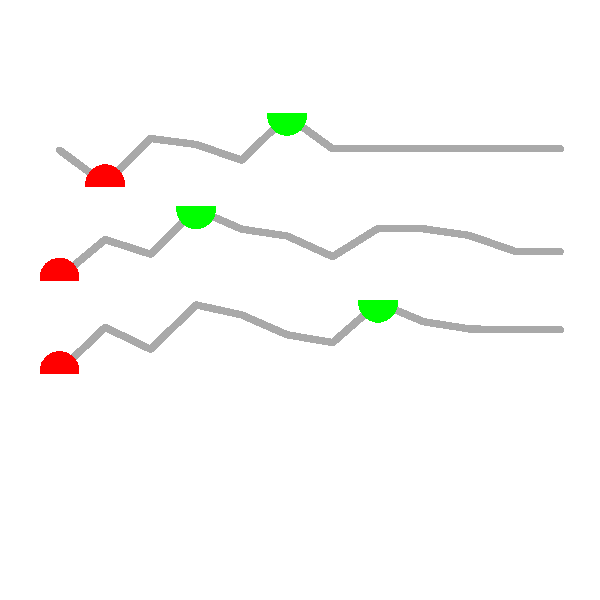
\includegraphics[width=\maxwidth]{figure/createSparklines_invest-1} 

}



      \vspace*{-0.5cm}
    \end{minipage}
    
    %\vspace*{-0.4cm}
    \begin{minipage}[c]{0.875\textwidth}
      \begin{flushleft}  
      {\color{white!30!blue} \textbf{\small Trade Indicators}}
      \end{flushleft} 
      \vspace*{-0.4cm}
      % Table 2
      \centering
      \resizebox{\textwidth}{!}{
% latex table generated in R 3.2.2 by xtable 1.7-4 package
% Wed May 25 16:26:55 2016
{\Large
\begin{tabular}{>{\raggedright}p{6in}r>{\raggedleft}p{0.8in}>{\raggedleft}p{0.8in}>{\raggedleft}p{0.8in}>{\raggedleft}p{0.8in}>{\raggedleft}p{0.8in}l}
  & Avg 2003-2012 & 2013 & 2014 & 2015 & 2016 & 2017 &  \\ 
  \hline
Total Trade in Goods and Services (\% of GDP, real terms) & 186.7 & 191.4 & 189.6 & 186.4 & 186.3 & 188.7 &  \\ 
  Trade balance (\% GDP, real terms) &  -7.1 & -11.2 & -11.4 &  -9.4 &  -9.8 &  -9.3 &  \\ 
  Exports, Goods and Services, annual percent change (real terms) &   7.9 &   5.5 &   5.5 &   3.5 &   4.5 &   7.3 &  \\ 
  Imports, Goods and Services, annual percent change (real terms) &   8.8 &   5.9 &   5.9 &   1.5 &   5.0 &   6.5 &  \\ 
  Total reserves in months of imports \large{[1]} &   1.1 &   1.4 &   1.2 & --- & --- & --- &  \\ 
  \end{tabular}
}

      }
    \end{minipage}
    \begin{minipage}[c]{0.11\textwidth}
      \vspace*{+0.8cm}


{\centering 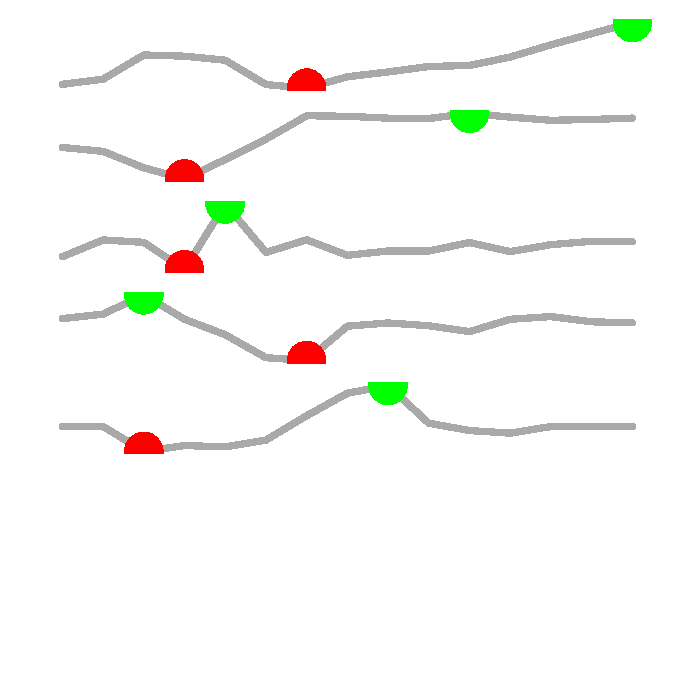
\includegraphics[width=\maxwidth]{figure/createSparklines_trade-1} 

}



      \vspace*{-0.4cm}
    \end{minipage}
  \\[3pt]
\raggedright{\footnotesize{\href{http://www.worldbank.org/en/topic/macroeconomics/overview}{Sources: MFM note}{,} \href{http://data.worldbank.org/data-catalog/world-development indicators}{[1] World Development Indicators (WDI)}{,} \href{http://unctadstat.unctad.org/wds/ReportFolders/reportFolders.aspx}{[2] UNCTADSTAT}{,} \href{https://www.imf.org/external/pubs/ft/weo/2015/02/weodata/index.aspx}{[3] World Economic Outlook (WEO)}}}
  \end{minipage} 
%\end{minipage}    
  \begin{minipage}[b]{\textwidth} % macro charts
  \vspace{+3ex}
    \begin{minipage}[c]{0.49\textwidth} % imports/exports 
    \center{\color{blue!50!black} \textbf{\small Goods Export and Import \\ volume growth, 2012-2015}}


{\centering 
\includegraphics[width=\maxwidth]{figure/ExpImp_HF-1} 

}



    \vspace*{-0.3cm}
    %\hspace*{0.5cm} 
    \raggedright{\footnotesize{\href{http://web.worldbank.org/WBSITE/EXTERNAL/EXTDEC/EXTDECPROSPECTS/0,,menuPK:476941~pagePK:51084723~piPK:51084722~theSitePK:476883,00.html}{Source: Development Prospects Group (DECPG)}}}
    \end{minipage}
    \begin{minipage}[c]{0.49\textwidth} % gdp value added
    \center{\color{blue!50!black} \textbf{\small Gross Value Added by \\ Economic Activity 2013 \footnotesize(\% GDP)}}


{\centering 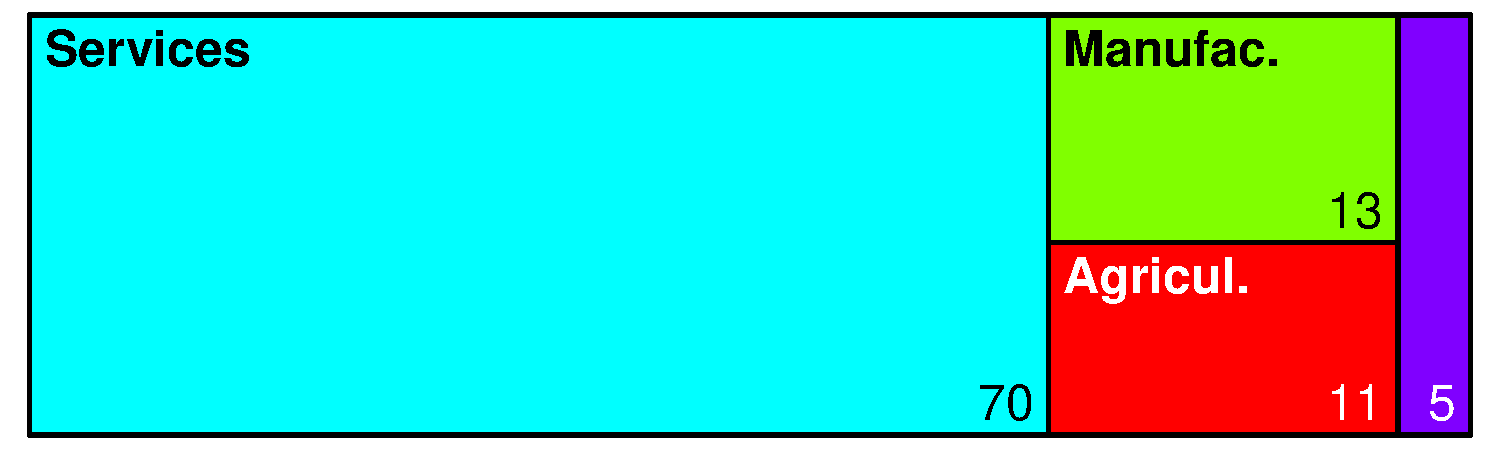
\includegraphics[width=\maxwidth]{figure/GVA_Treemap-1} 

}



   %\vspace*{-0.3cm}
   %\hspace*{0.5cm} 
   \raggedright{\footnotesize{\href{http://data.worldbank.org/data-catalog/world-development indicators}{Source: World Development Indicators (WDI)}}}
    \end{minipage}
  \end{minipage}  
\end{minipage}   
 
%%%% Exports Imports and DB
\begin{minipage}[b]{0.99\textwidth}
  \vspace{0.8cm}
   \begin{minipage}[c]{0.44\textwidth} 
    %\vspace*{-0.2cm}
    \begin{minipage}[t]{0.99\textwidth} 
      {\color{blue!50!black} \textbf{\small Top 5 Exports by \% of Total Value, NA}}
      %\vspace{3ex}
      \\[6pt]
      \centering
      \resizebox{\textwidth}{!}{%


{\centering 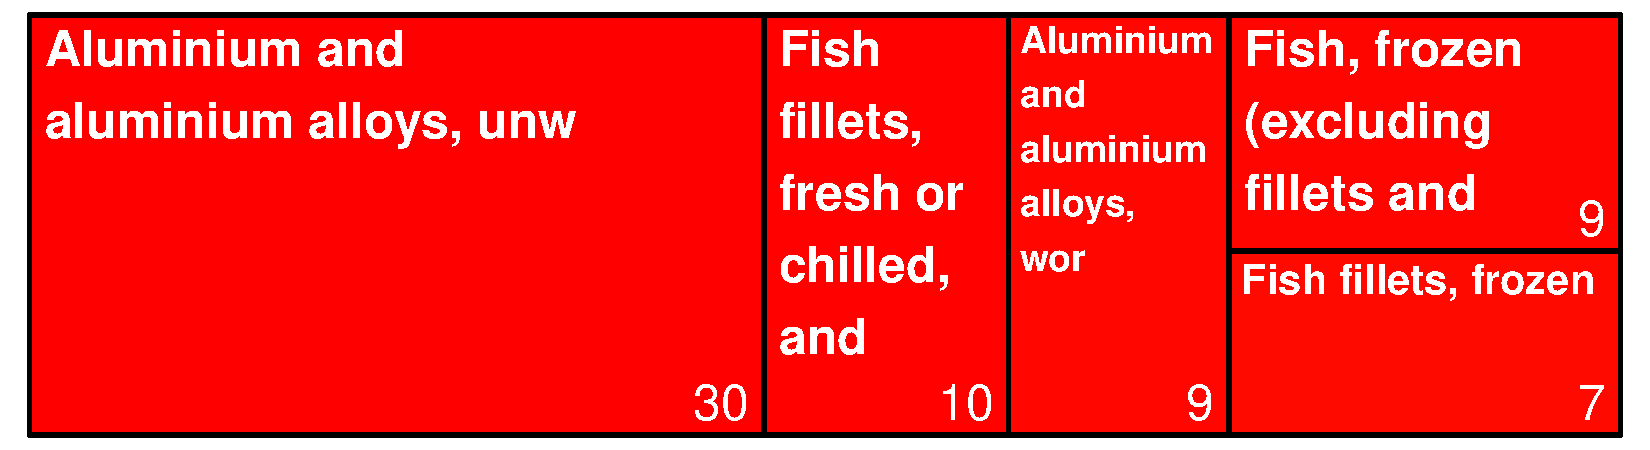
\includegraphics[width=\maxwidth]{figure/ImpExp_Treemap-2-1} 

}



      }
      \end{minipage}
      \\[14pt]
      \begin{minipage}[t]{0.99\textwidth} 
      {\color{blue!50!black} \textbf{\small Imports Categories by \% of Total Value, NA}}
      \\[6pt]
      \centering
      \resizebox{\textwidth}{!}{%


{\centering 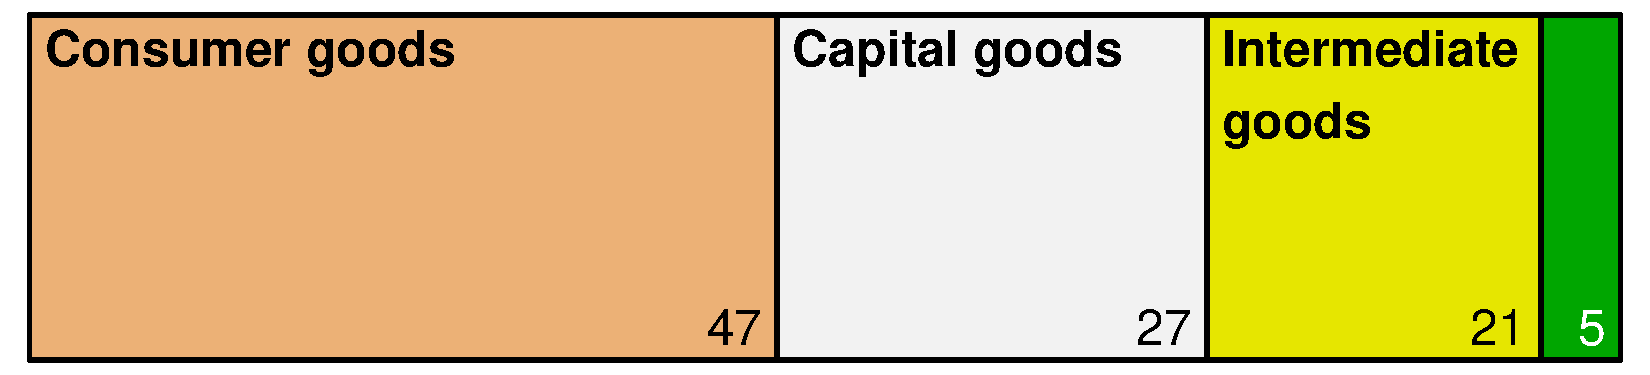
\includegraphics[width=\maxwidth]{figure/ImpExp_Treemap-1-1} 

}



      }
      \end{minipage}
      \\[10pt]
    %\hspace*{0.5cm}
    \footnotesize{\href{http://wits.worldbank.org}{Source: World Integrated Trade Solution (WITS)}} 
    \end{minipage}
    \begin{minipage}[c]{0.56\textwidth} % Doing Business table
    %\vspace*{-0.1cm}
    %\begin{flushleft}
      \center {\color{blue!50!black}\textbf{\small Doing Business 2015 \\ \footnotesize Distance to Frontier (DTF) and Rank}}
    %\end{flushleft}
    \\[18pt]
    \centering
      \resizebox{\textwidth}{!}{%
% latex table generated in R 3.2.2 by xtable 1.7-4 package
% Wed May 25 16:26:56 2016
{\large
\begin{tabular}{lrrr|rrrr}
  &  & DTF &  &  & Rank &  &  \\ 
  &  2015 &  2016 &  Change & 2015 & 2016 & Change &  \\ 
   \hline
\textbf{Ease of Doing Business} & \textbf{51.37} & \textbf{54.19} & \textbf{\color{green}{2.82}} & \textbf{138} & \textbf{132} & \textbf{\color{green}{6}} &  \\ 
  Dealing with Construction Permits & 57.9 & 57.98 & \color{green}{0.08} & 150 & 152 & \color{red}{-2} &  \\ 
  Enforcing Contracts & 63.49 & 63.49 & 0 & 54 & 54 & 0 &  \\ 
  Getting Credit & 35 & 40 & \color{green}{5} & 118 & 109 & \color{green}{9} &  \\ 
  Getting Electricity & 34.59 & 34.79 & \color{green}{0.2} & 176 & 177 & \color{red}{-1} &  \\ 
  Paying Taxes & 38.83 & 43.53 & \color{green}{4.7} & 178 & 172 & \color{green}{6} &  \\ 
  Protecting Minority Investors & 65 & 65 & 0 & 27 & 29 & \color{red}{-2} &  \\ 
  Registering Property & 60.29 & 60.78 & \color{green}{0.49} & 101 & 102 & \color{red}{-1} &  \\ 
  Resolving Insolvency & 29.26 & 29.04 & \color{red}{-0.22} & 147 & 147 & 0 &  \\ 
  Starting a Business & 85.76 & 90.26 & \color{green}{4.5} & 81 & 57 & \color{green}{24} &  \\ 
  Trading Across Borders & 43.59 & 57.05 & \color{green}{13.46} & 159 & 132 & \color{green}{27} &  \\ 
  \end{tabular}
}

      }
    \\[15pt]
     %\hspace*{0.5cm} 
     \raggedright{\footnotesize{\href{http://www.doingbusiness.org/data}{Source: Doing Busines Report 2015}}}
    \end{minipage}
\end{minipage}

\vspace{+3ex}
{\color{blue!50!white}\noindent\makebox[\linewidth]{\rule{18cm}{0.3pt}}} % horiz line
\begin{minipage}[c]{0.99\textwidth}
  \hspace*{-0.4cm}\raggedleft{\color{white!40!black} \footnotesize TRADE AND COMPETITIVENESS MONITORING NOTE - UPDATED 2016-05-25}
\end{minipage}

\newpage
%%%%%%%%%%%%%%%% PAGE 2 %%%%%%%%%%%%%%%%%%%

\begin{minipage}[t]{0.99\textwidth}
  \vspace{0.5cm}
  \begin{minipage}[c]{0.48\textwidth} % WEF Radar
    \center{\color{blue!50!black} \textbf{WEF Competitiveness Indicators \\ \footnotesize(Scale 1-7, 7=best)}}
    \vspace*{-0.6cm}


{\centering 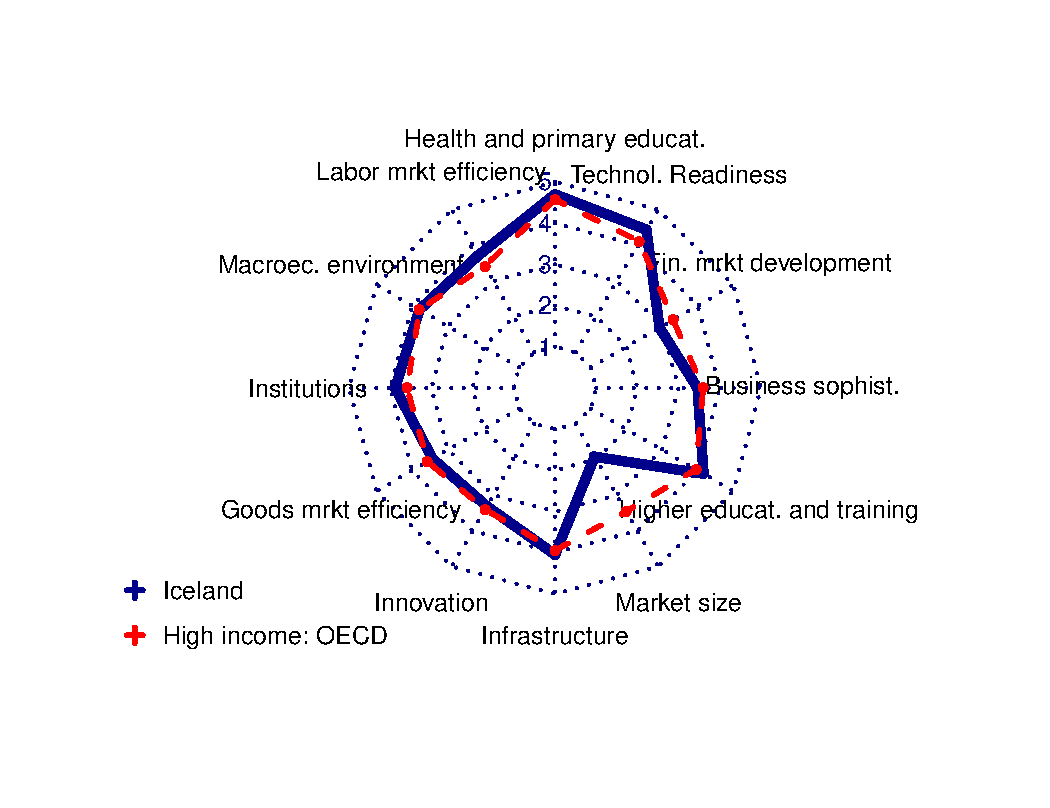
\includegraphics[width=\maxwidth]{figure/WEFradar-1} 

}



    \vspace*{-0.6cm} 
    \hspace*{0.3cm} \raggedright\footnotesize{\href{http://www.weforum.org/global-competitiveness-report-2015-2016}{Source: WEF Global Competitiveness Report 2015}}
  \end{minipage}
  \begin{minipage}[c]{0.50\textwidth} % LPI chart
  %\vspace*{0.5cm}
  \center {\color{blue!50!black} \textbf{Logistics Performance Index \\ \footnotesize(Scale 1-5, 5=best)}}
    \vspace*{0.4cm}


{\centering 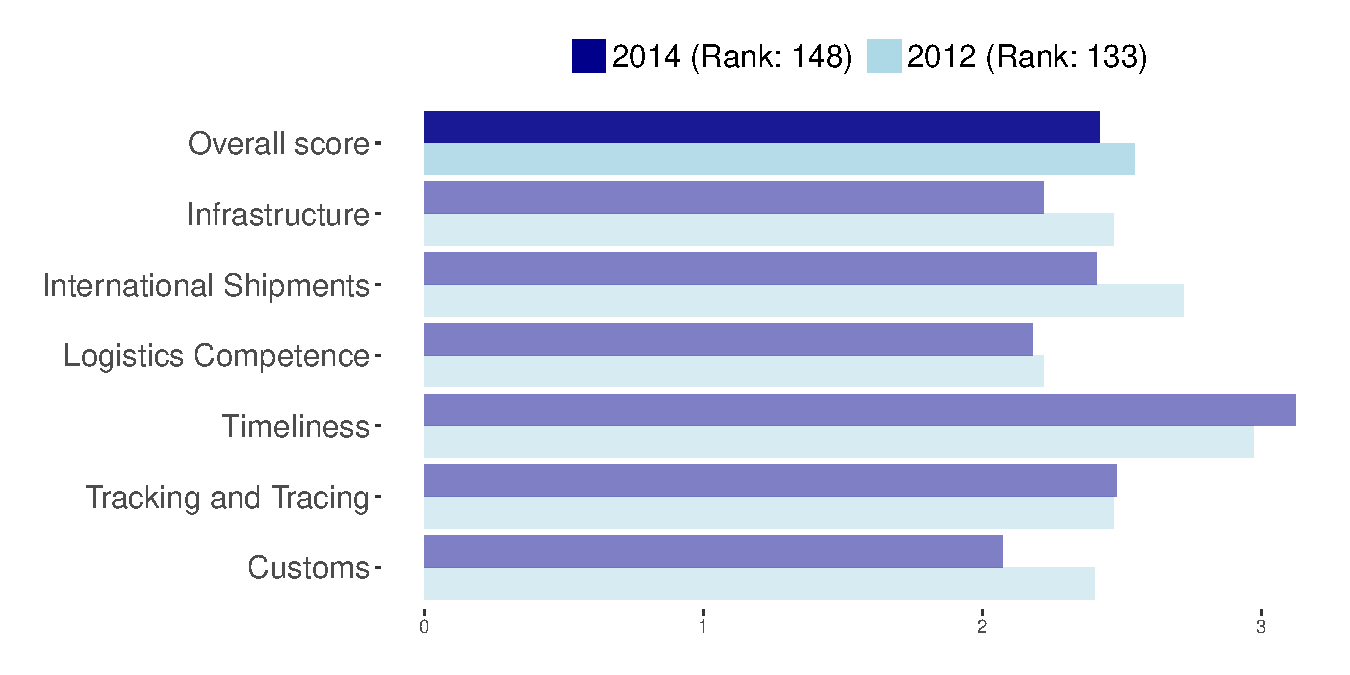
\includegraphics[width=\maxwidth]{figure/LPIindicators-1} 

}



  %\hspace*{0.5cm} 
  \raggedright\footnotesize{\href{http://lpi.worldbank.org}{Source: Logistics Performance Index (World Bank)}}
  \end{minipage}
\end{minipage}  

\begin{minipage}[b]{0.99\textwidth}
  \begin{minipage}[c]{0.50\textwidth} % WGI chart
    \vspace*{0.8cm}
    \center {\color{blue!50!black} \textbf{World Governance indicators \\ \footnotesize(Std. score, High=best)}}
    \vspace*{0.3cm}


{\centering 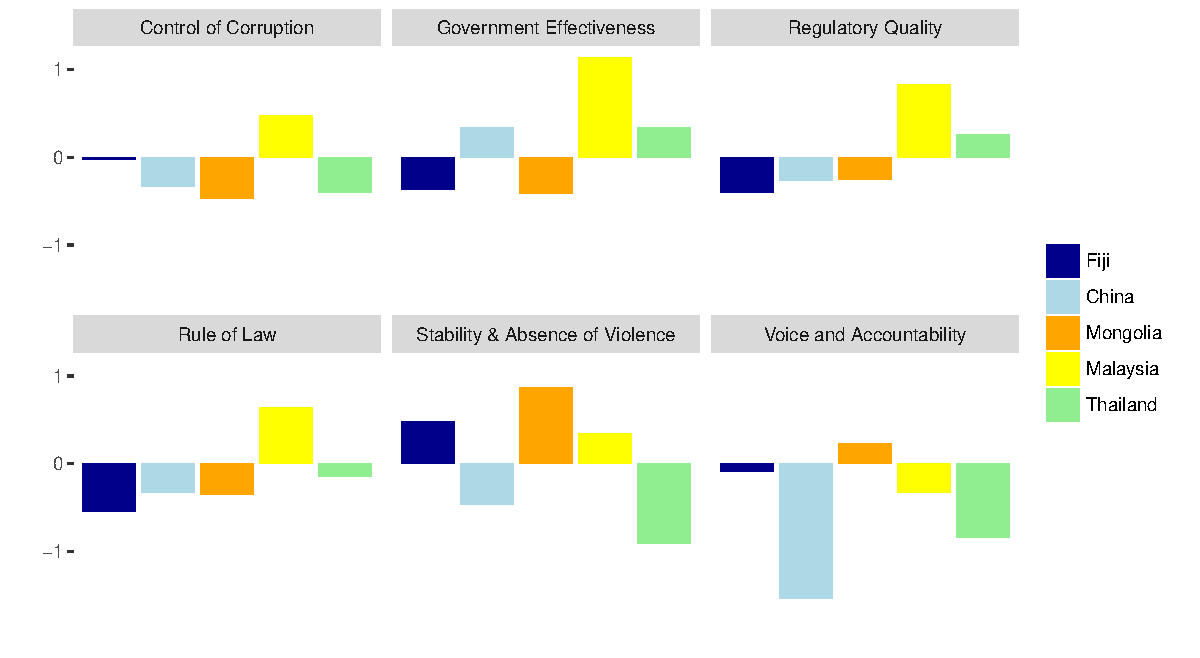
\includegraphics[width=\maxwidth]{figure/WGIindicators-1} 

}



    \vspace*{-0.6cm} 
    \hspace*{0.3cm} \raggedright\footnotesize{\href{http://data.worldbank.org/data-catalog/worldwide-governance-indicators}{Source: Worldwide Governance Indicators}}
  \end{minipage}
  \begin{minipage}[c]{0.48\textwidth} % Trade Policy table
    \vspace*{0.4cm}
  %\begin{flushleft}
    {\color{blue!50!black} \textbf{Trade Policy}}
  %\end{flushleft} 
  %\vspace*{0.2cm}
    \\[20pt]
    \centering
    \resizebox{\textwidth}{!}{%
% latex table generated in R 3.2.2 by xtable 1.7-4 package
% Wed May 25 16:26:57 2016
{\Large
\begin{tabular}{lrrr}
  & 2010 & 2015 &  \\ 
  \hline
Applied Tariff (Incl. Prefers. and Trade-Weighted) & 4.6 & 6.1 &  \\ 
  Binding (\%) & 100.0 & --- &  \\ 
  Dispersion (Standard Deviation) & 7.0 & 4.2 &  \\ 
  MFN Tariff (Agriculture) & 10.4 & 9.3 &  \\ 
  MFN Tariff (Non-Agriculture) & 7.3 & 7.1 &  \\ 
  MFN Tariff (Simple Average) & 7.8 & 7.5 &  \\ 
  \end{tabular}
}

    }
    \\[20pt]
    %\hspace*{0.5cm} 
    \raggedright{\footnotesize{\href{http://wits.worldbank.org}{Sources: WITS}{, }\href{http://stat.wto.org/CountryProfile/WSDBCountryPFHome.aspx?Language=E}{[1] WTO Trade Profiles}}}
  \end{minipage}
\end{minipage}

\vspace{+8ex}
%\hspace*{0.2cm}\subsection*{\color{white!50!black}Private Sector's Views}
\hspace*{0.1cm} \raggedright{\color{white!50!black}\Large Private Sector View}

\vspace*{-0.2cm}
{\color{white!30!black}\noindent\makebox[\linewidth]{\rule{18cm}{0.2pt}}} % horiz line

\begin{minipage}[b]{0.99\textwidth}
\vspace*{+0.6cm}
  \begin{minipage}[c]{0.02\textwidth}
  \hspace*{+0.1cm}
  \end{minipage}
  \begin{minipage}[c]{0.97\textwidth} 
    \begin{flushleft}  
      {\color{blue!50!black} \textbf{Enterprise Survey 2013}}
    \end{flushleft}  
    \vspace*{-0.4cm}
    \centering
    \resizebox{\textwidth}{!}{%
% latex table generated in R 3.2.2 by xtable 1.7-4 package
% Wed May 25 16:26:57 2016
{\Large
\begin{tabular}{lrrl}
  & All Countries & Tajikistan &  \\ 
  \hline
Number of electrical outages in a typical month & 6.30 & 6.10 &  \\ 
  Percent of firms with a bank loan/line of credit & 35.20 & 14.60 &  \\ 
  Proportion of investments financed by banks (\%) & 14.60 & 5.10 &  \\ 
  Proportion of investments financed internally (\%) & 71.20 & 73.90 &  \\ 
  Senior management time spent dealing with the requirements of government regulation (\%) & 10.00 & 21.90 &  \\ 
  \end{tabular}
}

    }
    \\[8pt]
    %\hspace*{0.3cm} 
    \raggedright{\footnotesize{\href{https://www.enterprisesurveys.org/data}{Source: Enterprise Survey 2013}}}
  \end{minipage} 

  \begin{minipage}[b]{0.99\textwidth} 
    \vspace{+4ex}
    \begin{minipage}[c]{0.49\textwidth} % top 5 constraints ES
      \center{\color{blue!50!black} \textbf{Top 5 constraints according to ES 2013 \\ \footnotesize(\% respondants)}}


{\centering 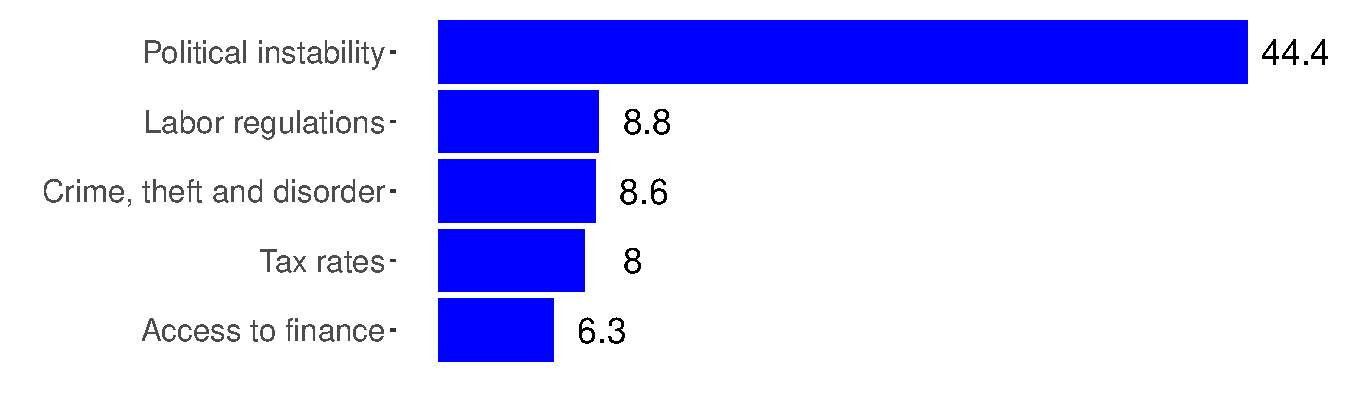
\includegraphics[width=\maxwidth]{figure/top5constraintsES-1} 

}



      %\vspace*{-0.7cm}
      \hspace*{0.3cm} \raggedright\footnotesize{\href{https://www.enterprisesurveys.org/data}{Source: Enterprise Survey 2013}}
    \end{minipage}
    \begin{minipage}[c]{0.49\textwidth} % top 5 constraints WEF
      \center{\color{blue!50!black} \textbf{Top 5 constraints according to WEF 2015 survey \\ \footnotesize(\% respondants among 88 executives)}}


{\centering 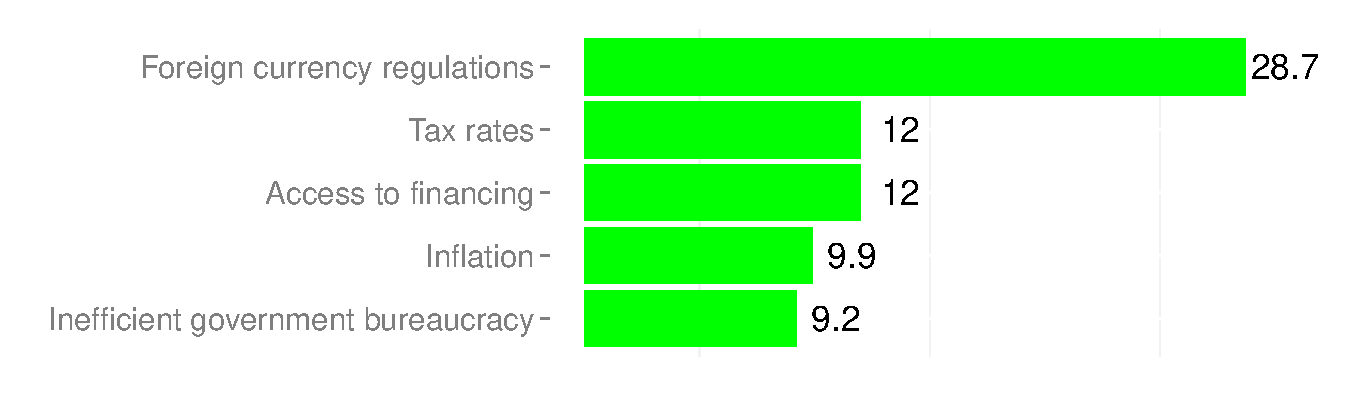
\includegraphics[width=\maxwidth]{figure/top5constraintsWEF-1} 

}



    %\vspace*{-0.7cm}
    \hspace*{0.3cm} \raggedright\footnotesize{\href{http://www.weforum.org/reports/global-competitiveness-report-2015-2016}{Source: WEF Global Competitiveness Report 2015}}
    \end{minipage}
  \end{minipage}
\end{minipage}

\vspace{+8ex}
{\color{blue!50!white}\noindent\makebox[\linewidth]{\rule{18cm}{0.3pt}}} % horiz line

\vspace{+2ex}
\begin{minipage}[c]{0.33\textwidth}
  \hspace*{+0.3cm} \includegraphics[width=4cm,left]{/Users/asanchez3/shinyTCMN/www/wb_logo.jpg}
  %\hspace*{+0.3cm} \includegraphics[width=4cm,left]{/Users/asanchez3/shinyTCMN/www/wb_logo.png}
\end{minipage}
\begin{minipage}[c]{0.65\textwidth}
  \vspace*{-0.4cm}
  \raggedleft{\color{white!40!black} \footnotesize TRADE AND COMPETITIVENESS MONITORING NOTE - UPDATED 2016-05-25}
\end{minipage}

%%%%%%%%%%%%%%%% END OF DOCUMENT %%%%%%%%%%%%%%%%%%%
\end{document}
